%----------------------------------------------------------------------------
\chapter{Other solutions}
\label{chap:relatedwork}
%----------------------------------------------------------------------------

It is important for a self-driving company to openly detail their technical
solution because it let's people trust their autopilot solution. However it
wasn't easy to find open information about the details of different companies,
because the technology itself is in early stages. The details I found did
provide inspiration on how to combine different algorithms. 

\section{Tesla}
The only open information I found about Tesla's autopilot technology is their
own keynote about autopilot \footnote{Tesla Autonomy Day
\url{https://www.youtube.com/watch?v=Ucp0TTmvqOE}}.


The sensor suite for tesla vehicles is seen on \autoref{fig:teslasensors}. Tesla uses 360\degree
RGB camera vision and sonar sensing with a radar facing forward. The sonar
sensors provide depth information for the surrounding objects and the radar
provides depth data for further distances.  

\begin{figure}[!ht]
  \centering
  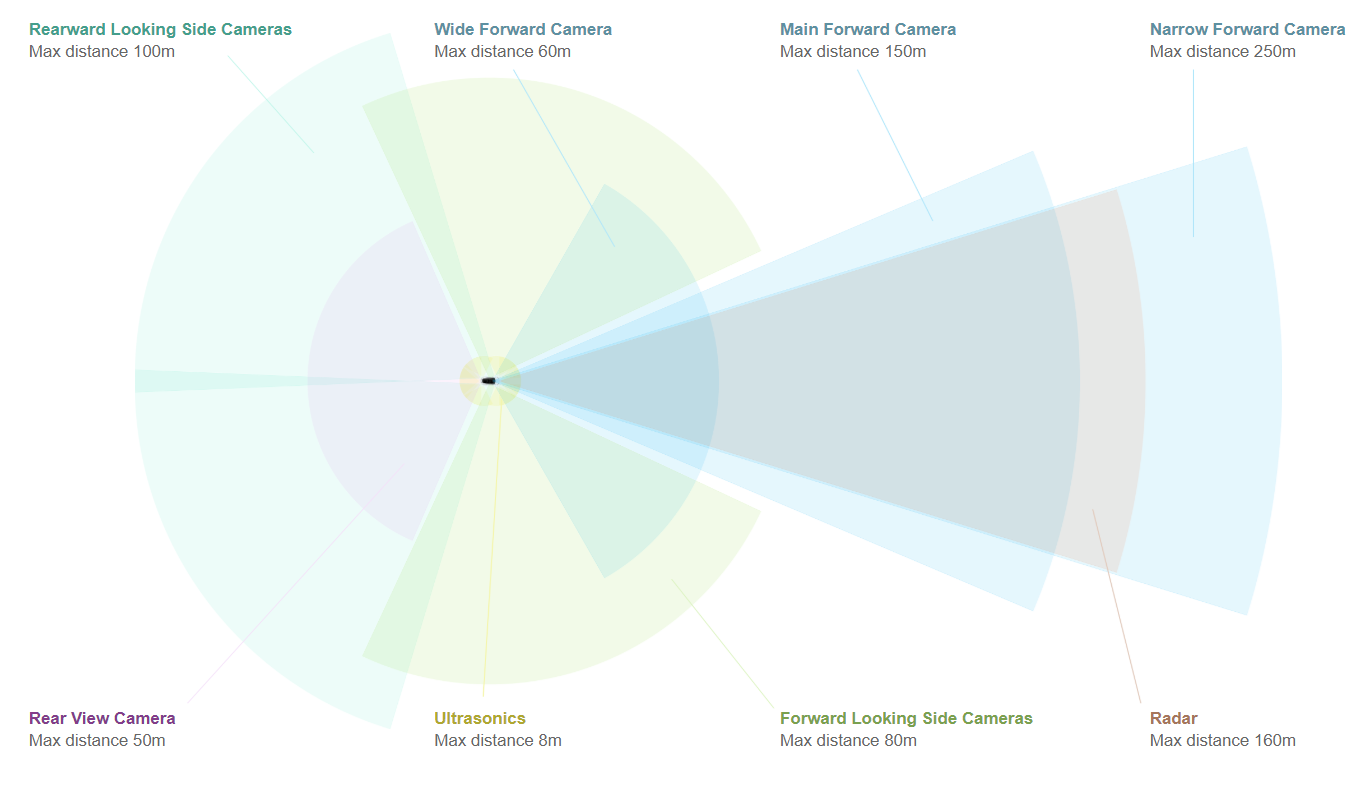
\includegraphics[width=150mm, keepaspectratio]{figures/teslasensors.png}
  \caption{Tesla sensor suite infographic from \url{https://www.tesla.com/autopilot}}
  \label{fig:teslasensors}
\end{figure}

The algorithms they use was not clear from the keynote, but they clearly
separate the following tasks.

\begin{itemize}
  \item Object detection
  \item Lane detection and path estimation
  \item Tracking
  \item Possibly some kind of segmentation
\end{itemize}

With sensor fusion they achieve depth estimation and detection thus they are able to
With sensor fusion they achieve depth estimation and detection thus they are able to
reconstruct the scenes around the vehicle.